%Beamer class
\documentclass{beamer}

\usepackage[czech]{babel}
\usepackage[cp1250]{inputenc}
\usepackage{fontenc}
\usepackage{tgheros}
\usepackage{array}
\usepackage{color}
\usepackage{hyperref}

\usetheme{Antibes}
\usecolortheme{crane}


\title[BE1M13VES]{BE1M13VES}
\subtitle[Manufacturing of Electrical Components] {Manufacturing of Electrical Components}
\author[Brejcha]{Michal Brejcha}
\institute[CTU]{CTU in Prague}
\date[Prague, 2017]{Prague, 2017}

\begin{document}
%------------------------------------------------------------------------------
%Uvodni slajd
%------------------------------------------------------------------------------
\frame{\titlepage}

\begin{frame}
\frametitle{Overview} 
\tableofcontents
\end{frame}

\AtBeginSection[]
{
  \begin{frame}
    \frametitle{TOPIC}
    \tableofcontents[currentsection]
  \end{frame}
}

%------------------------------------------------------------------------------
%Frquency dependency of resistors
%------------------------------------------------------------------------------
\section{\texorpdfstring{Photodiode}{Photodiode}}
%------------------------------------------------------------------------------
	\begin{frame}
    \frametitle{Semiconductor Components}
		\textbf{Basic properties}
		\begin{itemize}
		\item Nonlinear characteristics - used for rectifying, sensing, saturation etc.
		\item VA characteristics are quite dependent on ambient factors - temperature, light.
		\item Some components are able to amplify the input signal - transistors
		\end{itemize}
		
	\end{frame}
%------------------------------------------------------------------------------
%Diodes
%------------------------------------------------------------------------------
\section{\texorpdfstring{Solar Cells}{Solar Cells}}
%------------------------------------------------------------------------------
	%\begin{frame}
    %\frametitle{Diode}
		%The construction contain one junction between different types of semiconductor conductivity $\Rightarrow$ PN junction.
		%\begin{center}
			%\begin{tabular}{m{0.48\linewidth} m{0.42\linewidth}}
			%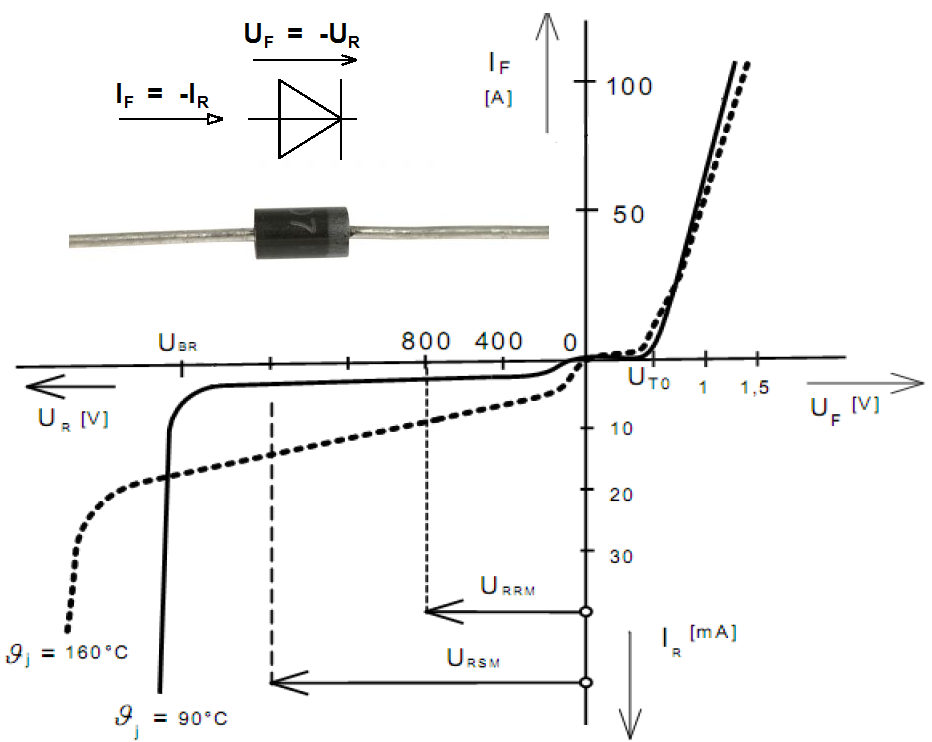
\includegraphics[scale=0.20]{obr04_dioda.png} &
			%Shockley diode equation
			%$$I = I_0\cdot\left(e^{\frac{U}{n\cdot U_T}}-1\right)$$
			%\small
			%\begin{itemize}
				%\item[$I_0$] ... saturation current,
				%\item[$U_T$] ...thermal voltage $=kT/e$,
				%\item[$n$] ...emission coefficient $=\left\langle 1, 2\right\rangle$.
			%\end{itemize}
			%
			%\end{tabular}
		%\end{center}
	%\end{frame}
%------------------------------------------------------------------------------
\end{document}